\chapter{Evaluierung}

\anno{ca. 10 Seiten (4)} %Ref. hat 5

Nachdem im letzten Kapitel hauptsächlich Aspekte der praktischen Umsetzung für das WAF-System erläutert wurden, widmet sich dieses Kapitel der Überprüfung der gemachten Annahmen aus der Zielbeschreibung der Arbeit. Insbesondere die Frage nach möglichst aktuellen bzw. neuen Daten und der damit verbundenen Qualität soll damit beantwortet werden. Dazu werden zuerst die benutzten Werkzeuge und der Testaufbau beschrieben. 

\section{Werkzeuge}
Für den Testaufbau werden einige Grundkomponenten benötigt. 

\subsection{Die Laufzeit- und Entwicklungsumgebung}
Für den Betrieb der in dieser Arbeit verwendeten Werkzeuge, wie z.B. Anwendungsserver oder Buildtools, ist eine Java-Laufzeitumgebung notwendig. In den lokal ausgeführten Fällen wurde dafür das \emph{Java Development Kit} der Firma Oracle in der Version 17.0.1 verwendet. Die im CI/CD-Build-Cycle ausgeführten Tests und Werkzeuge nutzen hingegen das Eclipse Temurin JDK in der jeweils aktuellsten Version 11.x


\subsection{OWASP\textregistered  Zed Attack Proxy}
\label{ref:zap}

\emph{The world's most widely used web app scanner}\footnote{https://zaproxy.org}\\

Der Zed Attack Proxy (ZAP) wird genutzt um Web Anwendungen auf Sicherheitslücken zu untersuchen. Als sogenannter Proxy befindet sich diese Anwendung zwischen dem Endnutzer bzw. Browser und der zu testenden Anwendung. ZAP bietet dabei zwei verschiedene Anwendungsmodi an. Im passiven Modus \emph{begleitet} ZAP den Nutzer auf seinem Weg durch eine Anwendung und registriert sämtliche IT-sicherheitstechnischen Auffälligkeiten. Der Nutzer klickt sich durch seine Anwendung, ggf. auf einem vorher definierten Weg,  und erhält am Ende eine Übersicht möglicher Angriffswege. Des Weiteren kann dieses Werkzeug zur Aufzeichnung der HTTP-Anfragen und -Antworten genutzt werden\\ Im aktiven Modus übernimmt ZAP selbst die Rolle des Angreifers und versucht Sicherheitslücken automatisch zu finden. \\

Es existieren zahlreiche weitere Tools mit ähnlicher Funktionalität, z.T. auch mit Spezialisierung auf das Testen von Web Application Firewalls. Nennenswerte Beispiele sind \emph{BurpSuite}, \emph{WAFNinja}, \emph{gotestwaf} und \emph{w3af}.  

\subsection{Web Server}

Zur Auslieferung der verwendeten Webapplikationen wird ein Web Server benötigt. Bedingt aus den Anforderungen der zu testenden Webanwendungen und Web Application Firewall muss dieser die Java Servlet Spezifikation implementieren. Bei der Verwendung eines lokalen Web Servers oder in den automatisierten Tests dieser Arbeit wird dabei der Apache Tomcat-Server in der Version 8.5.78 genutzt. Die Ausführung von Anwendungen die auf dem \emph{Spring}-Framework basieren benötigen nicht zwingend einen dedizierten Anwendungsserver, da diese ein integriertes System mit sich bringen (Undertow 2.2.18).

\subsection{Die Web Application Firewall}
Bei WebCastellum handelt es sich um eine Web Application Firewall die zum Schutz von Webanwendungen vor allgemeineren Angriffsszenarien entwickelt wurde. Implementiert wurde WebCastellum als ServletFilter, d.h. im Gegensatz zu WAF-Lösungen die als Proxy vor der Anwendung filtern, hätte WebCastellum vollen Zugriff auf alle Informationen die auch der Webanwendung bekannt sind. Erwähnenswert wären hier zum Beispiel der Login- oder Sessionstatus. 


\subsection{Ziel - Anwendungen}

\ref{sec:zieldesdatensatzes}

\subsubsection{PrimeFacesShowcase}

Beim PrimeFaces Showcase\footnote{Download unter https://www.primefaces.org/downloads} handelt es sich um eine Web-Anwendung zur Demonstration der PrimeFaces-Komponenten-Bibliothek. Dabei handelt es sich um eine Sammlung an Komponenten entsprechend der JSF-Spezifikation (JavaServerFaces). Neben der einfachen Darstellung der Komponenten liefert der Showcase auch Quelltext-Beispiele für deren Verwendung. Geht man davon aus dass eine Mehrheit der Entwickler diese Beispiele für eigene Implementierungen nutzt, könnte man schlussfolgern dass zahlreiche Anwendungen sicherheitstechnisch ähnlich reagieren wie der Showcase und dieser stellvertretend hier für den Nachweis genutzt werden kann.\anno{zu kompliziert?} Des weiteren bietet der Showcase die Möglichkeit \emph{alle} Komponenten des Frameworks zu testen.

\subsubsection{PetStore}

\subsubsection{CargoTracker}

\subsubsection{Spring PetClinic}



\subsubsection{OWASP\textregistered WebGoat}

In Form eines IT-Sicherheitstutorials wurde mit dem WebGoat-Projekt eine \emph{absichtlich, unsichere Anwendung} geschaffen, die es \emph{interessierten Entwicklern erlaubt häufig vorkommende Schwachstellen in Java-basierten Anwendungen} zu testen \cite{owaspgoat}. Da es sich um ein Tutorial handelt sind alles Schwachstellen auch explizit benannt. Ein guter Scanner sollte in diesem Fall auch alle Schwachpunkte auffinden können. 


\section{Aufbau der Testumgebung}
% Aufbau der Messumgebung (1-2 Seiten)
%% Server/Betriebssystem
%% Datensätze
%% Anfragen
%% Systeme/Ansätze gegen die Sie sich vergleichen
%% Wie messen Sie? Methodik und Maßeinheiten?
%% Ist die Messung signifikant?
%% Hypothesen? Was erwarten Sie?

Sämtliche Tests in dieser Arbeit werden nach dem Muster aus Abbildung \ref{fig.pattern} aufgebaut. Ein \glqq Angreifer\grqq{} versucht einen Angriff auf das \glqq Opfer\grqq. Zum Vergleich folgt auf einen Test ohne \glqq Verteidiger\grqq{} immer ein gleicher Test mit Verteidiger.

\begin{figure}[bht]
  \begin{center}
    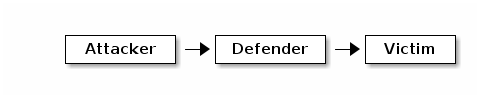
\includegraphics[width=10cm]{pattern}
    \caption{Muster für Tests}
    \label{fig.pattern}
  \end{center}
\end{figure}

\subsection{Attacker}
Angreifer können (handgeschriebene) Tests oder automatisierte Tools sein. Konkret werden in dieser Arbeit folgende Ausprägungen angewandt.

\subsubsection{Der manuelle Angriff}

Ein manueller Angriff ist ein exakt definierter Angriff der manuell ausgeführt wird. Der Ablauf ist dabei exakt in einer (Test-)Spezifikation beschrieben. Häufig existieren diese Tests in Form von Checklisten die vom einem Tester (Mensch) ab zuhaken sind. Mit Werkzeugen wie Selenium existieren auch Möglichkeiten diese Art von Test zu automatisieren. Der hier verwendete Test ruft im Grunde nur ein Formular auf und trägt in ein Textfeld einen mit einer SQl-Injektion versehenen bzw. manipulierten Wert ein. Im Anschluß wird das Formular abgesendet und der Rückgabewert kontrolliert.

\begin{neu}
manuellen Angriff beispielhaft erläutern; ggf. nochmal hinweis auf GrapheneTest (automatisierte Angriff); Hinweis/Übergang zu verschiedenen Beispiel-Datasets bzw. ref aus WAf-a-mole bzgl. verfügbarkeit
\end{neu}


\subsubsection{Der passive Angriff}
Im passiven Angriff wird der bereits aus Abschnitt \ref{ref:zap} bekannte \emph{Zed Attack Proxy} zwischen den Browser und der Webanwendung geschaltet. Im Grunde klickt sich nun ein Anwender durch die Anwendung und der Proxy ließt den Datenverkehr mit. Dabei werden die entdeckten Sicherheitslücken markiert. Um vergleichbare Ergebnisse zwischen den beiden Testläufen (mit und ohne aktiver Web Application Firewall) zu erhalten ist es zwingend erforderlich das beide Testläufe im Ablauf absolut gleich aufgebaut sind. Hierbei hilft beispielsweise die Definition des Testszenarios mittels Ablaufplan. Der Ablaufplan hilft auch bei einer späteren Automatisierung dieses Testvorgehens.

\subsubsection{Der aktive Angriff}
Beim aktiven Angriff übernimmt \emph{ZAP} die volle Kontrolle und sucht (möglichst) selbständig nach potentiellen Schwachstellen in der zugewiesenen Webanwendung. Eine \emph{kleine} Grundkonfiguration ist trotzdem notwendig, beispielsweise um Passworte zu hinterlegen falls ZAP - als Angreifer - auf eine Loginseite trifft. \\\\
\textcolor{bhtGray}{\ding{110} Hinweis} Ist man nicht Eigentümer der Ziel-Webanwendung sollte OWASP ZAPs aktiver Scanmodus nicht genutzt werden!\\


\subsection{Defender}

Hierbei handelt es sich um die zu testende Instanz der WebApplicationFirewall. Gegebenenfalls kann hier natürlich die Konfiguration - je nach Testfall - variieren. Da jedoch eine zentrale Installation im Fokus steht sollte in jedem Fall diese zentrale Instanz getestet werden.
% 3 Fälle -> ohne, defaultconfig, von zentrale gelieferte Konfiguration

\subsection{Victim}

Bei den \glqq\emph{Opfern}\grqq  im Test sollte es sich um zu schützende Anwendungen handeln. Vornehmlich sollte es sich um ein möglichst breit gefächertes Angebot an Anwendungen handeln. Aus zeitlichen Gründen werden in dieser Arbeit jedoch nur die im Grundlagen-Absatz erwähnten Anwendungen, \emph{Primefaces Showcase} und \emph{WebGoat} genutzt. Grundsätzlich könnten aber auch andere Anwendungen für den Testaufbau genutzt werden.\\ 

\subsection{TestMatrix}
Grundsätzlich besteht Bedarf möglichst viele Szenarien im Test abzudecken. Hierfür wird die in Tabelle \ref{tab:testplan} als Grundgerüst verwendet. Möglichst alle Angreifer sollten jeweils jedes Opfer angreifen. Mit steigender Anzahl an Opfern bzw. Tätern würde sich die Matrix entsprechend erweitern.

\anno{Tabelle müssen aktualisiert werden}
\begin{table}[h]
    \centering
    \begin{tabular}{cccc} 
      \toprule
    \textbf{Testlauf} & \textbf{Angreifer} & \textbf{Verteidiger} & \textbf{Opfer} \\ 
     \midrule
     1 & manuell & - & PF showcase\\
     2 & manuell & WebCastellum & PF showcase \\
     3 & ZAP (passiv) & - & PF showcase\\
     4 & ZAP (passiv) & WebCastellum & PF showcase \\
     5 & ZAP (aktiv) & - & PF showcase\\
     6 & ZAP (aktiv) & WebCastellum & PF showcase \\
     7 & manuell & - & WebGoat \\ 
    8 & manuell & WebCastellum & WebGoat \\
    9 & ZAP (passiv) & - & WebGoat \\ 
    10 & ZAP (passiv) & WebCastellum & WebGoat \\
    11 & ZAP (aktiv) & - & WebGoat \\ 
    12 & ZAP (aktiv) & WebCastellum & WebGoat \\
   \bottomrule
    \end{tabular}
    \caption{Testplan}
    \label{tab:testplan}
\end{table}

% Ergebnisse und Beobachtungen (3-4 Seiten)
\section{Ergebnisse und Beobachtungen}

% Beschreibung der Ergebnisse
% Diagramme
% Darstellen von Zusammenhängen

\anno{Tabellenwert! webgoat is spring ML lernen}

%lohnt es sich Training mit altem und neuen Datensatz zu testen? Zeit?

Die Ergebnisse aus den Tests (nach der spezifizierten Testmatrix) zeigen eine eindeutige Verbesserung durch Nutzung der Web Application Firewall. 

\begin{table}[h]
    \centering
    \begin{tabular}{cccccc} 
      \toprule
    \textbf{Testlauf} & \textbf{Angreifer} & \textbf{Verteidiger} & \textbf{Opfer} & \textbf{Schwachstellen} & \textbf{Verbesserung(in \%)} \\ 
     \midrule
     1 & manuell & - & PF showcase & 3 &\\
     2 & manuell & WebCastellum & PF showcase & 1 & 66\\
     3 & ZAP (passiv) & - & PF showcase & 16 &\\
     4 & ZAP (passiv) & WebCastellum & PF showcase & 2 & 87.5 \\
     5 & ZAP (aktiv) & - & PF showcase & 56 & \\
     6 & ZAP (aktiv) & WebCastellum & PF showcase & 20 & 64.3\\
     7 & manuell & - & WebGoat & 10 & \\ 
    8 & manuell & WebCastellum & WebGoat & 3 & 70 \\
    9 & ZAP (passiv) & - & WebGoat & 25 & \\ 
    10 & ZAP (passiv) & WebCastellum & WebGoat & 12 & 50\\
    11 & ZAP (aktiv) & - & WebGoat & 34 & \\ 
    12 & ZAP (aktiv) & WebCastellum & WebGoat & 14 & 59 \\
   \bottomrule
    \end{tabular}
    \caption{Ergebnisse}
    \label{tab:tes1tergebnisse}
  \end{table}

  Tabelle \ref{tab:tes1tergebnisse} gibt einen Überblick über die allgemeine Frage ob Angriffe verhindert werden können. Grundsätzlich verbessert der Einsatz einer WAF die IT-Sicherheit signifikant. Die zweite Tabelle verdeutlicht die Ergebnisse nochmals anhand der einzelnen Kategorien.

\begin{table}[h]
    \centering
    \begin{tabular}{cccccc} 
      \toprule
    \textbf{Testlauf} & \textbf{SQLi} & \textbf{CSRF} & \textbf{XMLi} & \textbf{sonstige} & \textbf{gesamt} \\ 
     \midrule
     1 & 2 & 1 &  &  & 3\\
     2 &   & 1 &  &  & 1\\
     3 & 6 & 5 &  & 5 & 16\\
     4 &   & 1 &  & 1  & 2 \\
     5 & 22 & 9 & 7 & 8& 56\\
     6 &  & 7 & 5 & 8 & 20 \\
     7 & 7 & 3 &  &  &  10  \\ 
    8 &  & 3 &  & & 3  \\
    9 & 11 & 5 &  & 9 & 25 \\ 
    10 &   & 5 &  & 7  & 12 \\
    11 & 17 & 8 &  & 9 & 34  \\ 
    12 &  & 8 &  & 6 & 14 \\
   \bottomrule
    \end{tabular}
    \caption{Ergebnisse}
    \label{tab:tes2tergebnisse}
\end{table}

Betrachtet man Tabelle \ref{tab:tes2tergebnisse} fällt auf das die Wirksamkeit der Firewall insbesondere im Fall von SQL-Injections (SQLi) gegeben ist. Nach Einsatz der Firewall wurden alle vorher erkannten Schwachstellen geschlossen bzw. eine Ausnutzung der Schwachstelle verhindert. Beide Anwendungen beinhalten eine oder mehrere Schwachpunkte im Bereich Cross-Site-Request-Forgery (CSRF). Obwohl die WAF-Software einen derartigen Schutzmechanismus beinhaltet scheint dieser nur im \emph{Primefaces Showcase} zum Teil zu wirken. Für die \emph{WebGoat}-Anwendung scheint dieser jedoch wirkungslos zu sein.


% Diskussion und Bewertung (3-4 Seiten)
\section{Bewertung}

% Wurden Sie überrascht?
% Stimmten die Hypothesen?
% Sind sie besser, anders als das andere System?
% wichtigster Erkenntnisgewinn?
% Anwendbarkeit Szenario?


% Zusammenfassung: ca. 0,5 Seiten


\section{Zusammenfassung}

% Was haben wir in diesem Kapitel gelernt?
% Wie passt das zur Zielstellung der Arbeit?
% Wie passt das zum nächsten Kapitel?